\subsubsection{2.1. Các thông số cho huấn luyện và kiểm thử}

\paragraph{2.1.1. Tham số mô hình, siêu tham số và kỹ thuật huấn luyện}
\indent\indent Về cấu hình tham số, đề tài áp dụng chiến lược đóng băng toàn bộ kiến trúc CNN backbone trong việc huấn luyện baseline và huấn luyện mô hình MGAT + FastKAN. Ngoài ra, mô hình ngôn ngữ all-MiniLM-L6-v2 cũng được sử dụng ở chế độ đóng băng để trích xuất đặc trưng văn bản. Do đó, tổng số lượng tham số (Total Params) của hệ thống bao gồm cả phần đóng băng và phần có thể huấn luyện (Trainable Params). Chi tiết thống kê tham số cho từng kịch bản cụ thể như sau:

\vspace{0.3cm}
%===================================================================
\textbf{* CNN Baseline:}
\begin{table}[H]
    \centering
    \caption{Thống kê số lượng tham số của các mô hình CNN Baseline}
    \label{tab:CNNBaselineParams}
    \renewcommand{\arraystretch}{1.15}
    \begin{tabular}{lcccc}
        \hline
        \textbf{Mô hình} & \textbf{Trainable Params} & \textbf{Total Params} \\
        \hline
        ResNet18              & 4.1K & 11.2M \\
        RegNetX400MF          & 3.2K & 5.1M \\
        MobileNetV3 Large     & 7.7K & 3.0M \\
        MobileNetV3 Small     & 4.6K & 1.0M \\
        DenseNet121           & 8.2K & 7.0M \\
        ShuffleNetV2 1.0x     & 8.2K & 1.3M \\
        \hline
    \end{tabular}
\end{table}

%===================================================================
\newpage
\textbf{* CNN backbone + MGAT + FastKAN/MLP:}
\begin{table}[H]
    \centering
    \renewcommand{\arraystretch}{1.2}
    \setlength{\tabcolsep}{6pt}
    \caption{\centering Thống kê số lượng tham số của mô hình CNN backbone + MGAT + FastKAN/MLP}
    \begin{tabular}{llcccc}
        \hline
        \textbf{Backbone Model (+ MGAT)} & \textbf{Classifier} & \textbf{Trainable Params} & \textbf{Total Params} \\
        \hline
        % ResNet18
        \multirow{2}{*}{ResNet18} 
        & FastKAN & 4.9M & 38.8M \\
        & MLP & 4.1M & 38.0M \\
        \hline
        % RegNetX400MF
        \multirow{2}{*}{RegNetX400MF} 
        & FastKAN & 4.9M & 32.7M \\
        & MLP & 4.1M & 31.9M \\
        \hline
        % MobileNetV3 Large
        \multirow{2}{*}{MobileNetV3 Large} 
        & FastKAN & 5.1M & 30.8M \\
        & MLP & 4.3M & 30.0M \\
        \hline
        % MobileNetV3 Small
        \multirow{2}{*}{MobileNetV3 Small} 
        & FastKAN & 5.0M & 28.6M \\
        & MLP & 4.2M & 27.8M \\
        \hline
        % DenseNet121
        \multirow{2}{*}{DenseNet121} 
        & FastKAN & 5.2M & 34.8M \\
        & MLP & 4.4M & 34.0M \\
        \hline
        % ShuffleNetV2
        \multirow{2}{*}{ShuffleNetV2 1.0x} 
        & FastKAN & 5.2M & 29.1M \\
        & MLP & 4.4M & 28.3M \\
        \hline
    \end{tabular}
    \label{tab:PipelineFullParams}
\end{table}

%===================================================================
\textbf{* Các siêu tham số và kỹ thuật huấn luyện:}
Quá trình huấn luyện được thực hiện thống nhất với bộ siêu tham số sau:
\begin{itemize}[label={--}, itemsep=1pt]
    \item Epoch: 100.
    \item Batch size: 8.
    \item Accumulation steps: 2 (Kỹ thuật tích lũy gradient này giúp mô phỏng kích thước batch thực tế là 16, cho phép mô hình hội tụ ổn định hơn mà vẫn tiết kiệm bộ nhớ VRAM)
    \item Early Stopping: Cơ chế dừng sớm được kích hoạt với patience = 10. Nếu sau 10 epoch liên tiếp giá trị \textit{validation loss} không cải thiện, quá trình huấn luyện sẽ tự động kết thúc.
    \item Optimizer: \textit{AdamW} với tốc độ học khởi tạo \textit{lr = 1e-4} và trọng số suy giảm \textit{weight\_decay = 1e-5}.
    \item Scheduler: Sử dụng chiến lược \textit{ReduceLROnPlateau} để tự động giảm tốc độ học (factor=0.5) nếu loss không giảm sau 3 epoch (patience=3).
    \item Drop Node (Augmentation): Để tăng khả năng tổng quát hóa của mô hình, tôi áp dụng kỹ thuật loại bỏ ngẫu nhiên các đỉnh ngay trong quá trình huấn luyện. Quy trình bao gồm 2 lượt drop liên tiếp:
    \begin{itemize}[label={+}, itemsep=1pt]
        \item Hình ảnh: Lần 1 (tỷ lệ 0.2), Lần 2 (tỷ lệ 0.3).
        \item Văn bản: Lần 1 (tỷ lệ 0.3), Lần 2 (tỷ lệ 0.4). Đặc biệt, áp dụng ràng buộc min\_not\_drop = 10 để đảm bảo mỗi mẫu luôn giữ lại ít nhất 10 từ khóa quan trọng, tránh làm mất mát hoàn toàn ngữ nghĩa của mô tả.
        \item Âm thanh: Lần 1 (tỷ lệ 0.2), Lần 2 (tỷ lệ 0.3).
    \end{itemize}
    Tỷ lệ drop cao hơn được áp dụng cho văn bản vì số lượng đỉnh của phương thức này chiếm đa số trong đồ thị và có độ biến động cao, trong khi số lượng đỉnh hình ảnh và âm thanh là cố định (lần lượt là 15 hình ảnh và 12 đoạn âm thanh). Thống kê phân bố số lượng từ trong tập huấn luyện được thể hiện tại \textbf{Hình \ref{fig:ThongKeTongSoTu}} và \textbf{Hình \ref{fig:ThongKeTBSoTu}}.
\end{itemize}

\begin{figure}[H]
    \centering
    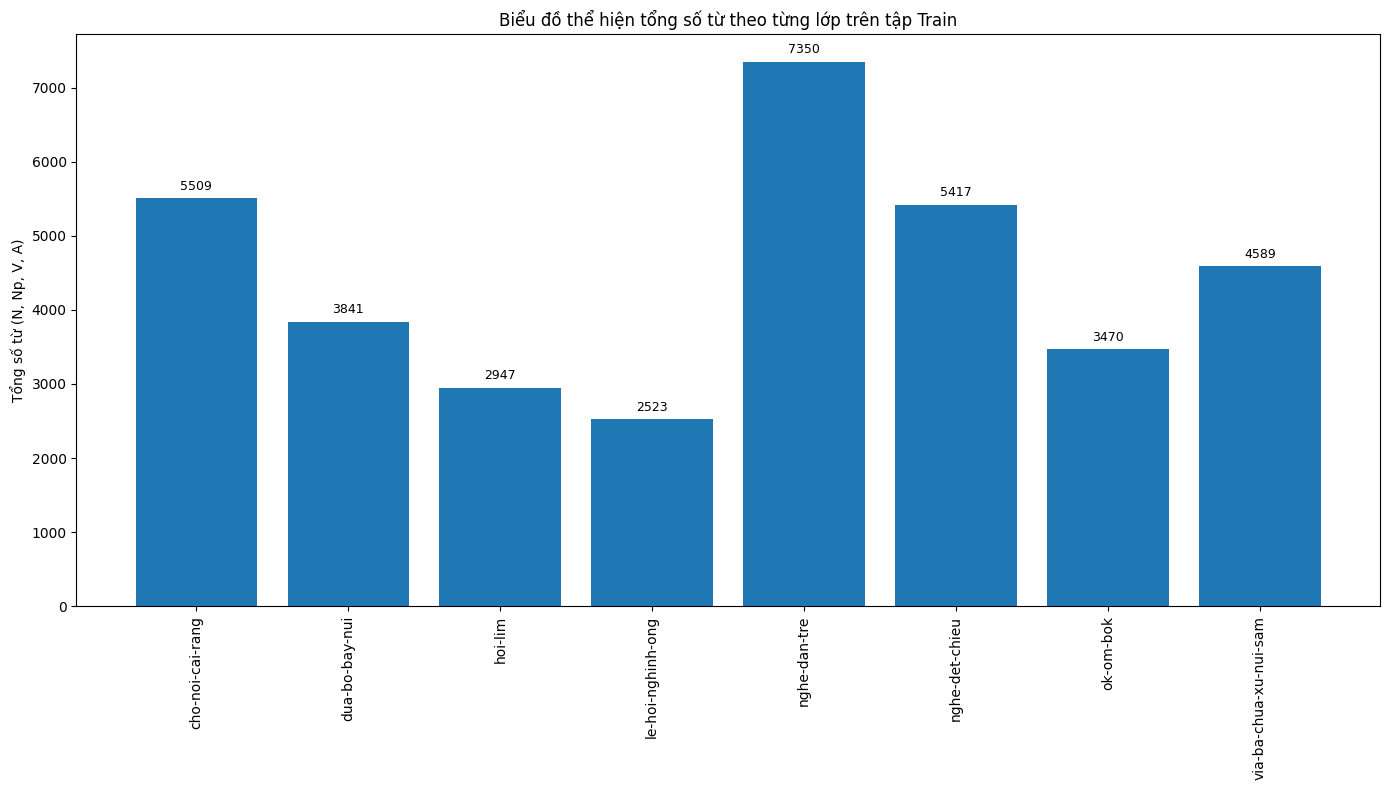
\includegraphics[width=0.9\linewidth]{images/part-02/chap-03/sec-02/ThongKeTongSoTu.png}
    \caption{Biểu đồ thống kê tổng số từ vựng trên tập Train}
    \label{fig:ThongKeTongSoTu}
\end{figure}
\begin{figure}[H]
    \centering
    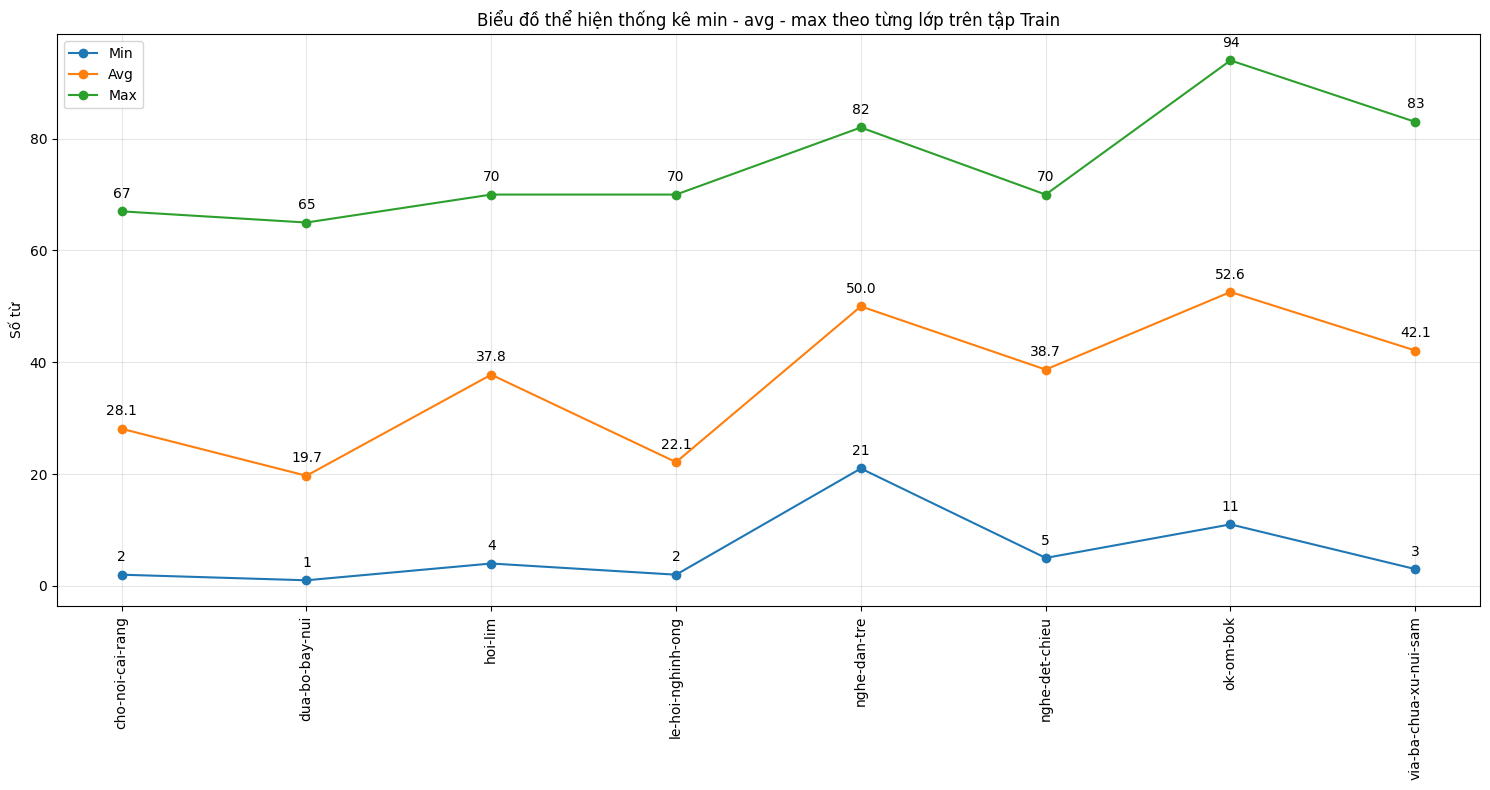
\includegraphics[width=0.9\linewidth]{images/part-02/chap-03/sec-02/ThongKeTBSoTu.png}
    \caption{Biểu đồ thống kê số lượng từ (Min, Avg, Max) trên tập Train}
    \label{fig:ThongKeTBSoTu}
\end{figure}

\paragraph{2.1.2. Chiến lược kiểm thử}
\indent\indent Quy trình kiểm thử tuân thủ nguyên tắc best model checkpoint. Trong quá trình huấn luyện, tại cuối mỗi epoch, nếu giá trị \textit{val\_loss < best\_val\_loss}, trạng thái trọng số của mô hình sẽ được lưu lại. Khi quá trình huấn luyện kết thúc (do hoàn thành 100 epoch hoặc early stopping), hệ thống sẽ tải lại phiên bản trọng số tốt nhất này để thực hiện đánh giá trên tập Test, đảm bảo kết quả phản ánh đúng năng lực của mô hình.\vspace{0.3cm}

Bên cạnh đó, nhằm đảm bảo tính khách quan và độ ổn định của quá trình huấn luyện cũng như các kết quả kiểm thử, đề tài sử dụng ba giá trị \textit{random seed} khác nhau, lần lượt là 1023, 123 và 42 (trong đó seed 42 được sử dụng cho kỹ thuật \textit{drop node}). Kết quả cuối cùng được báo cáo dưới dạng giá trị trung bình của ba lần huấn luyện và kiểm thử độc lập.